\documentclass[11pt,letterpaper]{article}
\usepackage{fullpage}
\usepackage[top=2cm, bottom=4.5cm, left=2.5cm, right=2.5cm]{geometry}
\usepackage{amsmath,amsfonts,amssymb}
\usepackage{lastpage}
\usepackage[inline]{enumitem}
\usepackage{fancyhdr}
\usepackage{mathrsfs}
\usepackage{xcolor}
\usepackage{graphicx}
\usepackage{hyperref}
\usepackage{subcaption}
\hypersetup{colorlinks=true, linkcolor=blue, linkbordercolor={0 0 1}}

\renewcommand{\arraystretch}{1.75}

\setlength{\parindent}{0.0in}
\setlength{\parskip}{0.05in}

\newcommand{\its}{\item[\tiny\textbullet]}

\pagestyle{fancyplain}
\lhead{Brad Cownden}
\chead{}
\rhead{June 25, 2020}
\cfoot{\small\thepage}
\headsep 36pt

\begin{document}
\vspace{.2in}
\begin{center}
    {\bf GPU Solutions for PSCAD: IT17112}
\end{center}

\vspace{.25in}

\begin{tabular}{| p{0.2\textwidth} | p{0.75\textwidth} |}
	\hline
	Reporting Period & June 18, 2020 - June 25, 2020 \\ \hline

	Activities & \begin{enumerate*}
    \item[\tiny\textbullet]  Profiled GPU use during the execution of \texttt{QRFactor} on the Quadro RTX 3000 card \newline
    \its During execution, there were three primary kernel calls to the GPU that were of particular importance: 
        \begin{enumerate*} 
            \item  ``csrqr\_leftLooking\_cta\_byLevels\_core'', called once during the 
            factoring of the matrix $A$ into the product $QR$, 
            \item ``csrqr\_solve\_Qtb\_cta\_core'', called to compute $Q^{-1} \mathbf{b}(t)$
    at each time step, and
            \item ``csrqr\_upper\_direct\_kernel'', called to solve $R\mathbf{x}(t) = Q^{-1} \mathbf{b}(t)$ for $\mathbf{x}(t)$ at each time step
        \end{enumerate*} \newline
    \its Using NVIDIA Compute profiling tools, each kernel can be examined in great detail. See figure~\ref{f:kernel_profile} for
    a sample profile page \newline
    \its Extracted Total GPU Utilization and Achieved Occupancy values from each kernel. See table~\ref{t:gpu_profile} for values \newline
    \its High values for Achieved Occupancy signal efficient use of available warps in the Streaming Multiprocessor (SM) \newline
    \its While total GPU Utilization never exceeded 66\%, this figure can be misleading. In the Compute Workload Analysis portion 
    of figure~\ref{f:kernel_profile} we see a breakdown of utilization of the each type of resource that the SM is capable 
    of using. Since the Quadro RTX 3000 is specialized towards graphics rendering, there are fewer resources available 
    at the hardware level for the double-precision operations required by \texttt{QRFactor}. Depending on the choice of hardware, more FP64 resources may
    be available, leading to a lower total GPU Utilization.
    \end{enumerate*} \\ \hline

	Issues & \begin{enumerate*}
	\item[\tiny\textbullet] None
	\end{enumerate*} \\ \hline

	Milestones \newline Accomplished & \begin{enumerate*}
	\item[\tiny\textbullet] Profiling of \texttt{QRFactor} on Quadro RTX 3000 \newline
    \end{enumerate*} \\ \hline

	Milestones Not \newline Accomplished & \begin{enumerate*}
	\item[\tiny\textbullet] None
	\end{enumerate*} \\ \hline

	Next Week's \newline Milestones & \begin{enumerate*}
    \item[\tiny\textbullet] Examine effects of scaling the size of the problem on P100 and V100 hardware
	\end{enumerate*} \\ \hline

	Forwarded Issues & \begin{enumerate*}
	\item[\tiny\textbullet] None
	\end{enumerate*} \\ \hline
\end{tabular}

\vspace{.25in}

\begin{table}[ht]
    \centering
    \begin{tabular}{| c | c | c |}
        \hline
        {\bf Kernel} & {\bf Total GPU Utilization \%} & {\bf Achieved Occupancy \%}  \\ \hline
        csrqr\_leftLooking\_cta\_byLevels\_core & 65.7 & 92.7 \\ \hline
        csrqr\_solve\_Qtb\_cta\_core & 14.5 & 99.2 \\ \hline
        csrqr\_upper\_direct\_kernel & 40.1 & 75.7 \\ \hline
    \end{tabular}
    \caption{Profiling information for the three major kernel calls in \texttt{QRFactor}.}
    \label{t:gpu_profile}
\end{table}


\begin{figure}[!ht]
    \centering
    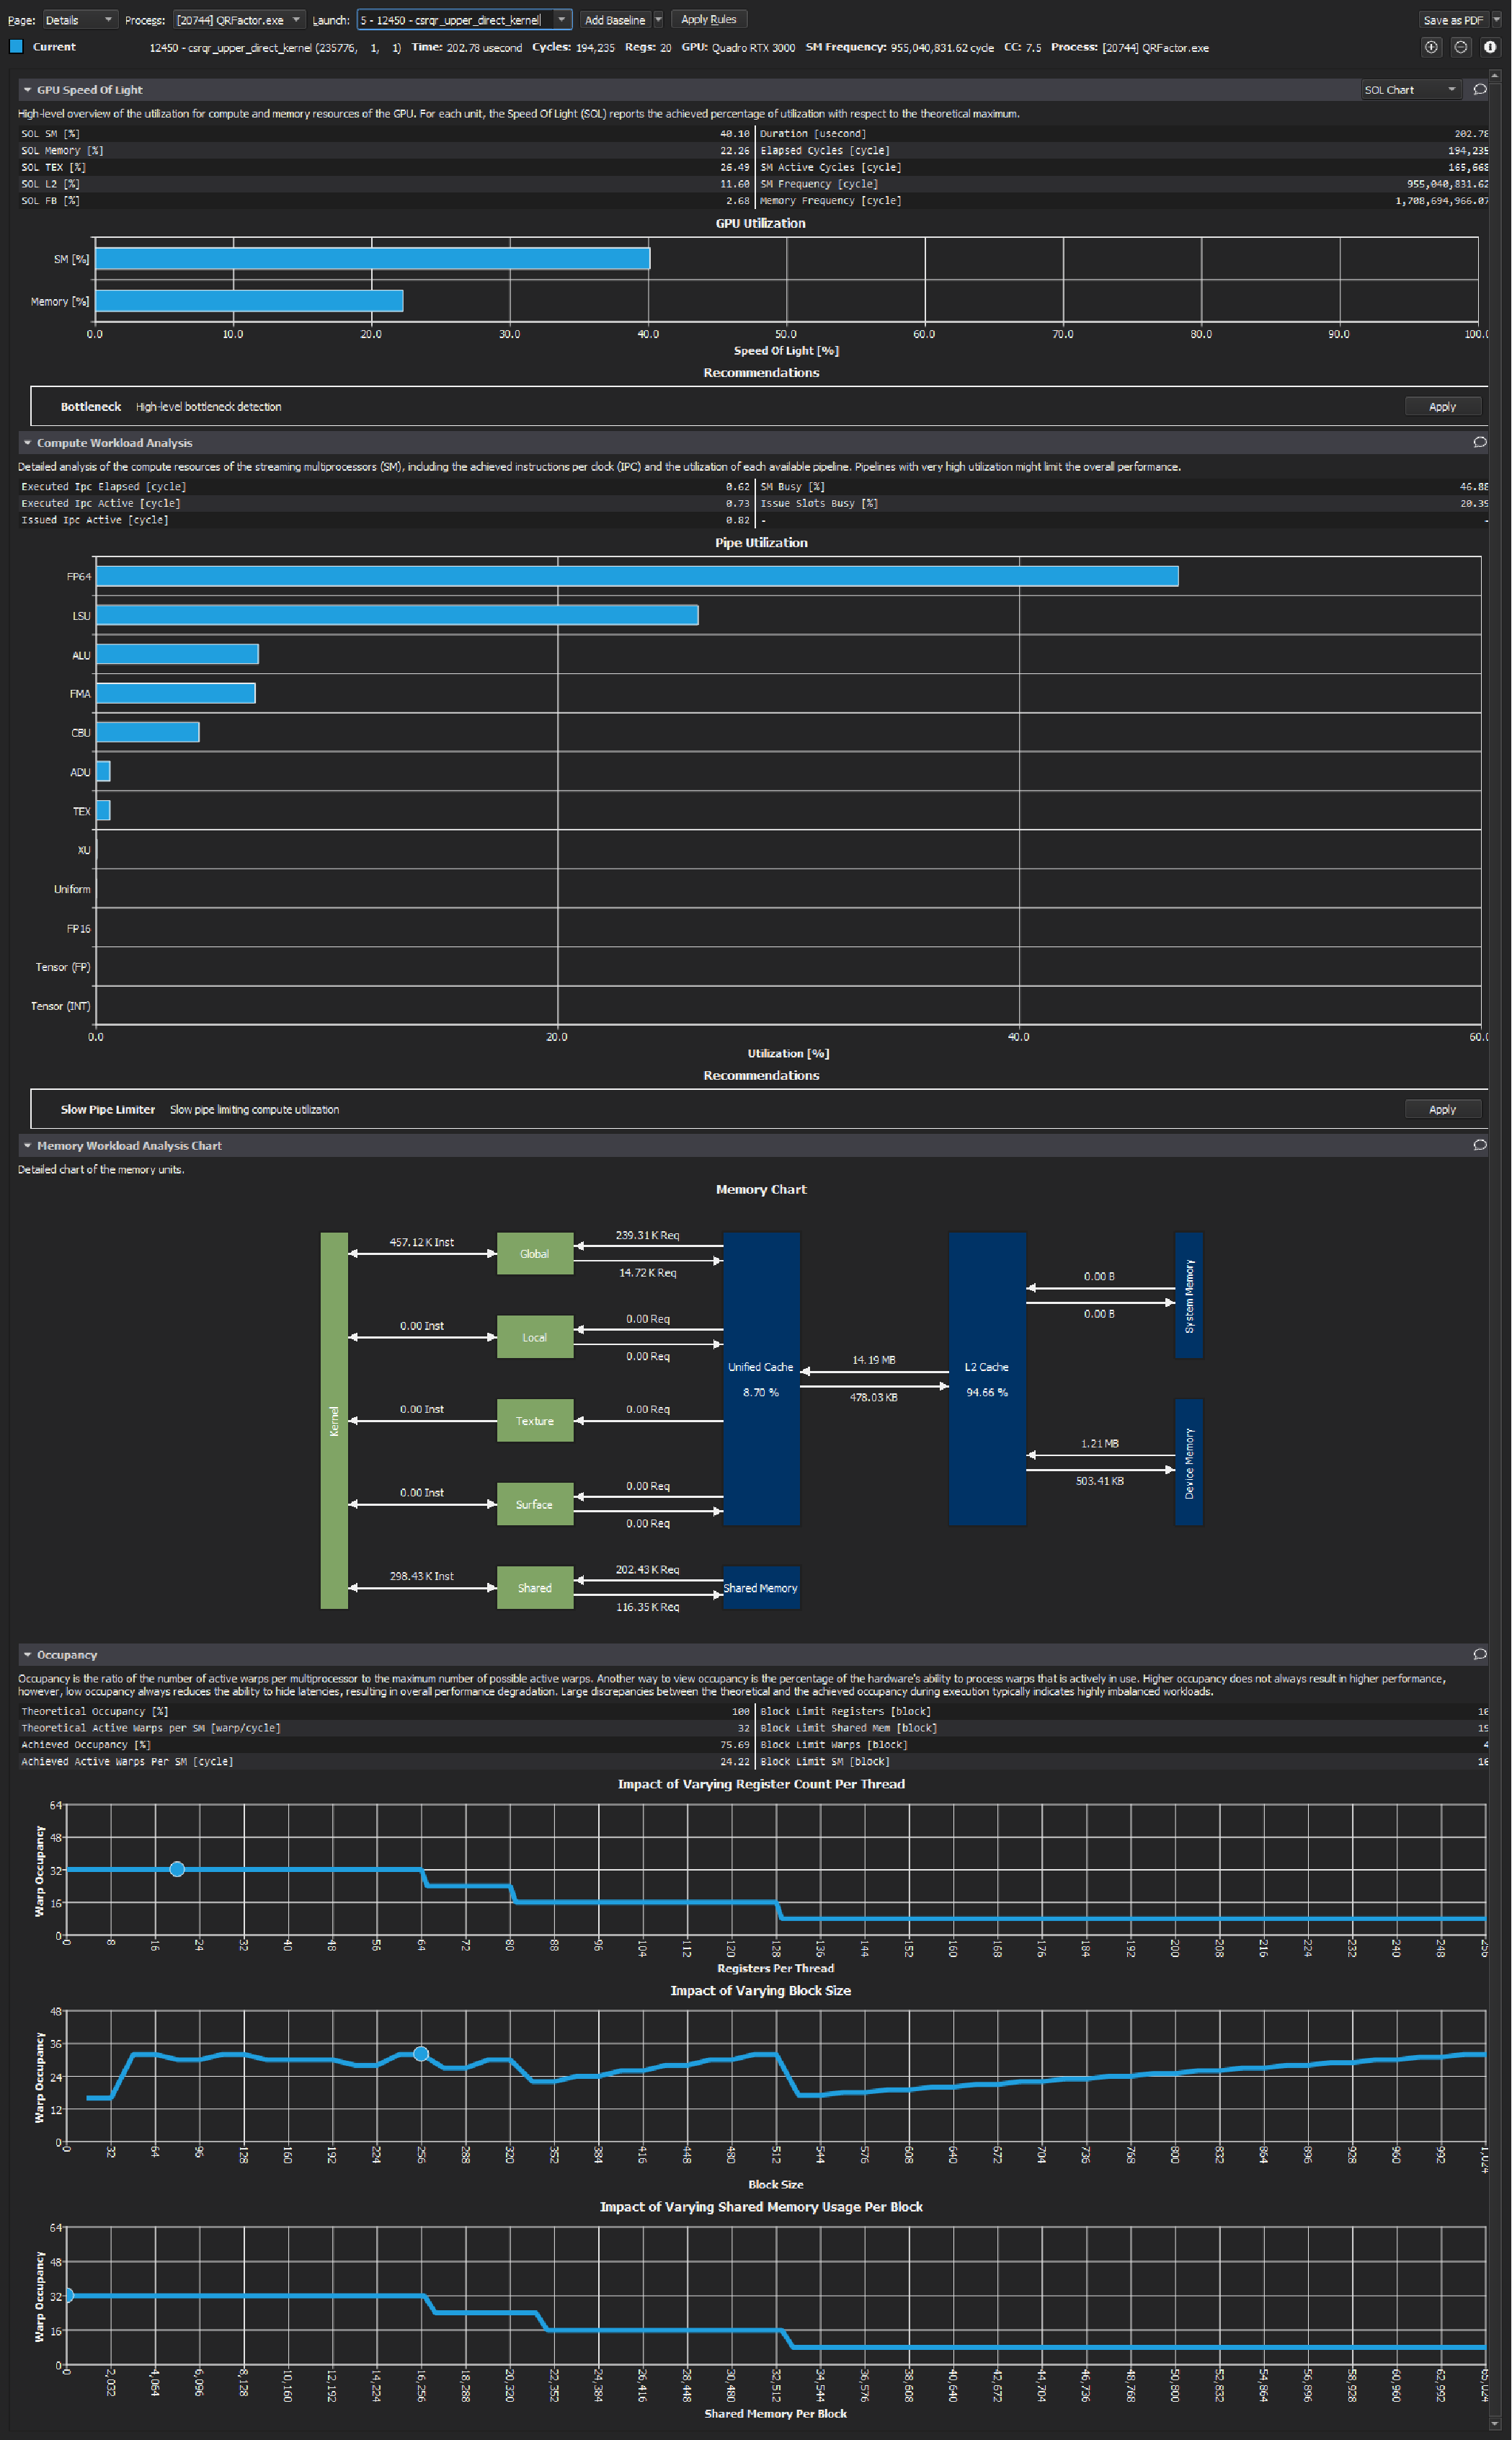
\includegraphics[width=0.75\textwidth]{C:/Users/bradc/Documents/MHI/Reports/kernel_profile.pdf}
    \caption{An example of the full profile for a kernel call using NVIDIA Compute.}
    \label{f:kernel_profile}
\end{figure}

\end{document}
